\documentclass[10pt,a4paper,onecolumn]{article}
\usepackage{marginnote}
\usepackage{graphicx}
\usepackage[rgb,svgnames]{xcolor}
\usepackage{authblk,etoolbox}
\usepackage{titlesec}
\usepackage{calc}
\usepackage{tikz}
\usepackage[pdfa]{hyperref}
\usepackage{hyperxmp}
\hypersetup{%
    unicode=true,
    pdfapart=3,
    pdfaconformance=B,
    pdftitle={maze-dataset: Maze Generation with Algorithmic Variety and
Representational Flexibility},
    pdfauthor={Michael Igorevich Ivanitskiy, Aaron Sandoval, Alex F.
Spies, Tilman Räuker, Brandon Knutson, Cecilia Diniz Behn, Samy Wu
Fung},
    pdfpublication={Journal of Open Source Software},
    pdfpublisher={Open Journals},
    pdfissn={2475-9066},
    pdfpubtype={journal},
    pdfvolumenum={},
    pdfissuenum={},
    pdfdoi={10.xxxxxx/draft},
    pdfcopyright={Copyright (c) 1970, Michael Igorevich Ivanitskiy,
Aaron Sandoval, Alex F. Spies, Tilman Räuker, Brandon Knutson, Cecilia
Diniz Behn, Samy Wu Fung},
    pdflicenseurl={http://creativecommons.org/licenses/by/4.0/},
    colorlinks=true,
    linkcolor=[rgb]{0.0, 0.5, 1.0},
    citecolor=Blue,
    urlcolor=[rgb]{0.0, 0.5, 1.0},
    breaklinks=true
}
% https://tex.stackexchange.com/a/535849
% Create an OutputIntent in order to correctly specify colours
\immediate\pdfobj stream attr{/N 3} file{sRGB.icc}
\pdfcatalog{%
  /OutputIntents [
    <<
      /Type /OutputIntent
      /S /GTS_PDFA1
      /DestOutputProfile \the\pdflastobj\space 0 R
      /OutputConditionIdentifier (sRGB)
      /Info (sRGB)
    >>
  ]
}
\pdfvariable omitcidset=1
\usepackage{caption}
\usepackage{orcidlink}
\usepackage{tcolorbox}
\usepackage{amssymb,amsmath}
\usepackage{ifxetex,ifluatex}
\usepackage{seqsplit}
\usepackage{xstring}

\usepackage{float}
\let\origfigure\figure
\let\endorigfigure\endfigure
\renewenvironment{figure}[1][2] {
    \expandafter\origfigure\expandafter[H]
} {
    \endorigfigure
}

\usepackage{fixltx2e} % provides \textsubscript

% definitions for citeproc citations
\NewDocumentCommand\citeproctext{}{}
\NewDocumentCommand\citeproc{mm}{%
  \begingroup\def\citeproctext{#2}\cite{#1}\endgroup}
\makeatletter
 % allow citations to break across lines
 \let\@cite@ofmt\@firstofone
 % avoid brackets around text for \cite:
 \def\@biblabel#1{}
 \def\@cite#1#2{{#1\if@tempswa , #2\fi}}
\makeatother
\newlength{\cslhangindent}
\setlength{\cslhangindent}{1.5em}
\newlength{\csllabelwidth}
\setlength{\csllabelwidth}{3em}
\newenvironment{CSLReferences}[2] % #1 hanging-indent, #2 entry-spacing
 {\begin{list}{}{%
  \setlength{\itemindent}{0pt}
  \setlength{\leftmargin}{0pt}
  \setlength{\parsep}{0pt}
  % turn on hanging indent if param 1 is 1
  \ifodd #1
   \setlength{\leftmargin}{\cslhangindent}
   \setlength{\itemindent}{-1\cslhangindent}
  \fi
  % set entry spacing
  \setlength{\itemsep}{#2\baselineskip}}}
 {\end{list}}
\usepackage{calc}
\newcommand{\CSLBlock}[1]{\hfill\break\parbox[t]{\linewidth}{\strut\ignorespaces#1\strut}}
\newcommand{\CSLLeftMargin}[1]{\parbox[t]{\csllabelwidth}{\strut#1\strut}}
\newcommand{\CSLRightInline}[1]{\parbox[t]{\linewidth - \csllabelwidth}{\strut#1\strut}}
\newcommand{\CSLIndent}[1]{\hspace{\cslhangindent}#1}

% --- Page layout -------------------------------------------------------------
\usepackage[top=3.5cm, bottom=3cm, right=1.5cm, left=1.0cm,
            headheight=2.2cm, reversemp, includemp, marginparwidth=4.5cm]{geometry}

% --- Default font ------------------------------------------------------------
\renewcommand\familydefault{\sfdefault}

% --- Style -------------------------------------------------------------------
\renewcommand{\captionfont}{\small\sffamily}
\renewcommand{\captionlabelfont}{\bfseries}

% --- Section/SubSection/SubSubSection ----------------------------------------
\titleformat{\section}
  {\normalfont\sffamily\Large\bfseries}
  {}{0pt}{}
\titleformat{\subsection}
  {\normalfont\sffamily\large\bfseries}
  {}{0pt}{}
\titleformat{\subsubsection}
  {\normalfont\sffamily\bfseries}
  {}{0pt}{}
\titleformat*{\paragraph}
  {\sffamily\normalsize}


% --- Header / Footer ---------------------------------------------------------
\usepackage{fancyhdr}
\pagestyle{fancy}
\fancyhf{}
%\renewcommand{\headrulewidth}{0.50pt}
\renewcommand{\headrulewidth}{0pt}
\fancyhead[L]{\hspace{-0.75cm}
\includegraphics[width=5.5cm]{joss/logo.png}}
\fancyhead[C]{}
\fancyhead[R]{}
\renewcommand{\footrulewidth}{0.25pt}

\fancyfoot[L]{\parbox[t]{0.98\headwidth}{\footnotesize{\sffamily Ivanitskiy
et al. (2025). maze-dataset: Maze Generation with Algorithmic Variety
and Representational Flexibility. \emph{Journal of Open Source
Software}, \emph{¿VOL?}(¿ISSUE?), ¿PAGE?
\url{https://doi.org/10.xxxxxx/draft}}.}}


\fancyfoot[R]{\sffamily \thepage}
\makeatletter
\let\ps@plain\ps@fancy
\fancyheadoffset[L]{4.5cm}
\fancyfootoffset[L]{4.5cm}

% --- Macros ---------

\definecolor{linky}{rgb}{0.0, 0.5, 1.0}

\newtcolorbox{repobox}
   {colback=red, colframe=red!75!black,
     boxrule=0.5pt, arc=2pt, left=6pt, right=6pt, top=3pt, bottom=3pt}

\newcommand{\ExternalLink}{%
   \tikz[x=1.2ex, y=1.2ex, baseline=-0.05ex]{%
       \begin{scope}[x=1ex, y=1ex]
           \clip (-0.1,-0.1)
               --++ (-0, 1.2)
               --++ (0.6, 0)
               --++ (0, -0.6)
               --++ (0.6, 0)
               --++ (0, -1);
           \path[draw,
               line width = 0.5,
               rounded corners=0.5]
               (0,0) rectangle (1,1);
       \end{scope}
       \path[draw, line width = 0.5] (0.5, 0.5)
           -- (1, 1);
       \path[draw, line width = 0.5] (0.6, 1)
           -- (1, 1) -- (1, 0.6);
       }
   }

\definecolor{c53baa1}{RGB}{83,186,161}
\definecolor{c202826}{RGB}{32,40,38}
\def \rorglobalscale {0.1}
\newcommand{\rorlogo}{%
\begin{tikzpicture}[y=1cm, x=1cm, yscale=\rorglobalscale,xscale=\rorglobalscale, every node/.append style={scale=\rorglobalscale}, inner sep=0pt, outer sep=0pt]
  \begin{scope}[even odd rule,line join=round,miter limit=2.0,shift={(-0.025, 0.0216)}]
    \path[fill=c53baa1,nonzero rule,line join=round,miter limit=2.0] (1.8164, 3.012) -- (1.4954, 2.5204) -- (1.1742, 3.012) -- (1.8164, 3.012) -- cycle;
    \path[fill=c53baa1,nonzero rule,line join=round,miter limit=2.0] (3.1594, 3.012) -- (2.8385, 2.5204) -- (2.5172, 3.012) -- (3.1594, 3.012) -- cycle;
    \path[fill=c53baa1,nonzero rule,line join=round,miter limit=2.0] (1.1742, 0.0669) -- (1.4954, 0.5588) -- (1.8164, 0.0669) -- (1.1742, 0.0669) -- cycle;
    \path[fill=c53baa1,nonzero rule,line join=round,miter limit=2.0] (2.5172, 0.0669) -- (2.8385, 0.5588) -- (3.1594, 0.0669) -- (2.5172, 0.0669) -- cycle;
    \path[fill=c202826,nonzero rule,line join=round,miter limit=2.0] (3.8505, 1.4364).. controls (3.9643, 1.4576) and (4.0508, 1.5081) .. (4.1098, 1.5878).. controls (4.169, 1.6674) and (4.1984, 1.7642) .. (4.1984, 1.8777).. controls (4.1984, 1.9719) and (4.182, 2.0503) .. (4.1495, 2.1132).. controls (4.1169, 2.1762) and (4.0727, 2.2262) .. (4.0174, 2.2635).. controls (3.9621, 2.3006) and (3.8976, 2.3273) .. (3.824, 2.3432).. controls (3.7505, 2.359) and (3.6727, 2.367) .. (3.5909, 2.367) -- (2.9676, 2.367) -- (2.9676, 1.8688).. controls (2.9625, 1.8833) and (2.9572, 1.8976) .. (2.9514, 1.9119).. controls (2.9083, 2.0164) and (2.848, 2.1056) .. (2.7705, 2.1791).. controls (2.6929, 2.2527) and (2.6014, 2.3093) .. (2.495, 2.3487).. controls (2.3889, 2.3881) and (2.2728, 2.408) .. (2.1468, 2.408).. controls (2.0209, 2.408) and (1.905, 2.3881) .. (1.7986, 2.3487).. controls (1.6925, 2.3093) and (1.6007, 2.2527) .. (1.5232, 2.1791).. controls (1.4539, 2.1132) and (1.3983, 2.0346) .. (1.3565, 1.9436).. controls (1.3504, 2.009) and (1.3351, 2.0656) .. (1.3105, 2.1132).. controls (1.2779, 2.1762) and (1.2338, 2.2262) .. (1.1785, 2.2635).. controls (1.1232, 2.3006) and (1.0586, 2.3273) .. (0.985, 2.3432).. controls (0.9115, 2.359) and (0.8337, 2.367) .. (0.7519, 2.367) -- (0.1289, 2.367) -- (0.1289, 0.7562) -- (0.4837, 0.7562) -- (0.4837, 1.4002) -- (0.6588, 1.4002) -- (0.9956, 0.7562) -- (1.4211, 0.7562) -- (1.0118, 1.4364).. controls (1.1255, 1.4576) and (1.2121, 1.5081) .. (1.2711, 1.5878).. controls (1.2737, 1.5915) and (1.2761, 1.5954) .. (1.2787, 1.5991).. controls (1.2782, 1.5867) and (1.2779, 1.5743) .. (1.2779, 1.5616).. controls (1.2779, 1.4327) and (1.2996, 1.3158) .. (1.3428, 1.2113).. controls (1.3859, 1.1068) and (1.4462, 1.0176) .. (1.5237, 0.944).. controls (1.601, 0.8705) and (1.6928, 0.8139) .. (1.7992, 0.7744).. controls (1.9053, 0.735) and (2.0214, 0.7152) .. (2.1474, 0.7152).. controls (2.2733, 0.7152) and (2.3892, 0.735) .. (2.4956, 0.7744).. controls (2.6016, 0.8139) and (2.6935, 0.8705) .. (2.771, 0.944).. controls (2.8482, 1.0176) and (2.9086, 1.1068) .. (2.952, 1.2113).. controls (2.9578, 1.2253) and (2.9631, 1.2398) .. (2.9681, 1.2544) -- (2.9681, 0.7562) -- (3.3229, 0.7562) -- (3.3229, 1.4002) -- (3.4981, 1.4002) -- (3.8349, 0.7562) -- (4.2603, 0.7562) -- (3.8505, 1.4364) -- cycle(0.9628, 1.7777).. controls (0.9438, 1.7534) and (0.92, 1.7357) .. (0.8911, 1.7243).. controls (0.8623, 1.7129) and (0.83, 1.706) .. (0.7945, 1.7039).. controls (0.7588, 1.7015) and (0.7252, 1.7005) .. (0.6932, 1.7005) -- (0.4839, 1.7005) -- (0.4839, 2.0667) -- (0.716, 2.0667).. controls (0.7477, 2.0667) and (0.7805, 2.0643) .. (0.8139, 2.0598).. controls (0.8472, 2.0553) and (0.8768, 2.0466) .. (0.9025, 2.0336).. controls (0.9282, 2.0206) and (0.9496, 2.0021) .. (0.9663, 1.9778).. controls (0.9829, 1.9534) and (0.9914, 1.9209) .. (0.9914, 1.8799).. controls (0.9914, 1.8362) and (0.9819, 1.8021) .. (0.9628, 1.7777) -- cycle(2.6125, 1.3533).. controls (2.5889, 1.2904) and (2.5553, 1.2359) .. (2.5112, 1.1896).. controls (2.4672, 1.1433) and (2.4146, 1.1073) .. (2.3529, 1.0814).. controls (2.2916, 1.0554) and (2.2228, 1.0427) .. (2.1471, 1.0427).. controls (2.0712, 1.0427) and (2.0026, 1.0557) .. (1.9412, 1.0814).. controls (1.8799, 1.107) and (1.8272, 1.1433) .. (1.783, 1.1896).. controls (1.7391, 1.2359) and (1.7052, 1.2904) .. (1.6817, 1.3533).. controls (1.6581, 1.4163) and (1.6465, 1.4856) .. (1.6465, 1.5616).. controls (1.6465, 1.6359) and (1.6581, 1.705) .. (1.6817, 1.7687).. controls (1.7052, 1.8325) and (1.7388, 1.8873) .. (1.783, 1.9336).. controls (1.8269, 1.9799) and (1.8796, 2.0159) .. (1.9412, 2.0418).. controls (2.0026, 2.0675) and (2.0712, 2.0804) .. (2.1471, 2.0804).. controls (2.223, 2.0804) and (2.2916, 2.0675) .. (2.3529, 2.0418).. controls (2.4143, 2.0161) and (2.467, 1.9799) .. (2.5112, 1.9336).. controls (2.5551, 1.8873) and (2.5889, 1.8322) .. (2.6125, 1.7687).. controls (2.636, 1.705) and (2.6477, 1.6359) .. (2.6477, 1.5616).. controls (2.6477, 1.4856) and (2.636, 1.4163) .. (2.6125, 1.3533) -- cycle(3.8015, 1.7777).. controls (3.7825, 1.7534) and (3.7587, 1.7357) .. (3.7298, 1.7243).. controls (3.701, 1.7129) and (3.6687, 1.706) .. (3.6333, 1.7039).. controls (3.5975, 1.7015) and (3.5639, 1.7005) .. (3.5319, 1.7005) -- (3.3226, 1.7005) -- (3.3226, 2.0667) -- (3.5547, 2.0667).. controls (3.5864, 2.0667) and (3.6192, 2.0643) .. (3.6526, 2.0598).. controls (3.6859, 2.0553) and (3.7155, 2.0466) .. (3.7412, 2.0336).. controls (3.7669, 2.0206) and (3.7883, 2.0021) .. (3.805, 1.9778).. controls (3.8216, 1.9534) and (3.8301, 1.9209) .. (3.8301, 1.8799).. controls (3.8301, 1.8362) and (3.8206, 1.8021) .. (3.8015, 1.7777) -- cycle;
  \end{scope}
\end{tikzpicture}
}

% --- Title / Authors ---------------------------------------------------------
% patch \maketitle so that it doesn't center
\patchcmd{\@maketitle}{center}{flushleft}{}{}
\patchcmd{\@maketitle}{center}{flushleft}{}{}
% patch \maketitle so that the font size for the title is normal
\patchcmd{\@maketitle}{\LARGE}{\LARGE\sffamily}{}{}
% patch the patch by authblk so that the author block is flush left
\def\maketitle{{%
  \renewenvironment{tabular}[2][]
    {\begin{flushleft}}
    {\end{flushleft}}
  \AB@maketitle}}
\renewcommand\AB@affilsepx{ \protect\Affilfont}
%\renewcommand\AB@affilnote[1]{{\bfseries #1}\hspace{2pt}}
\renewcommand\AB@affilnote[1]{{\bfseries #1}\hspace{3pt}}
\renewcommand{\affil}[2][]%
   {\newaffiltrue\let\AB@blk@and\AB@pand
      \if\relax#1\relax\def\AB@note{\AB@thenote}\else\def\AB@note{#1}%
        \setcounter{Maxaffil}{0}\fi
        \begingroup
        \let\href=\href@Orig
        \let\protect\@unexpandable@protect
        \def\thanks{\protect\thanks}\def\footnote{\protect\footnote}%
        \@temptokena=\expandafter{\AB@authors}%
        {\def\\{\protect\\\protect\Affilfont}\xdef\AB@temp{#2}}%
         \xdef\AB@authors{\the\@temptokena\AB@las\AB@au@str
         \protect\\[\affilsep]\protect\Affilfont\AB@temp}%
         \gdef\AB@las{}\gdef\AB@au@str{}%
        {\def\\{, \ignorespaces}\xdef\AB@temp{#2}}%
        \@temptokena=\expandafter{\AB@affillist}%
        \xdef\AB@affillist{\the\@temptokena \AB@affilsep
          \AB@affilnote{\AB@note}\protect\Affilfont\AB@temp}%
      \endgroup
       \let\AB@affilsep\AB@affilsepx
}
\makeatother
\renewcommand\Authfont{\sffamily\bfseries}
\renewcommand\Affilfont{\sffamily\small\mdseries}
\setlength{\affilsep}{1em}


\ifnum 0\ifxetex 1\fi\ifluatex 1\fi=0 % if pdftex
  \usepackage[T1]{fontenc}
  \usepackage[utf8]{inputenc}

\else % if luatex or xelatex
  \ifxetex
    \usepackage{mathspec}
    \usepackage{fontspec}

  \else
    \usepackage{fontspec}
  \fi
  \defaultfontfeatures{Scale=MatchLowercase}
  \defaultfontfeatures[\sffamily]{Ligatures=TeX}
  \defaultfontfeatures[\rmfamily]{Ligatures=TeX,Scale=1}

\fi
% use upquote if available, for straight quotes in verbatim environments
\IfFileExists{upquote.sty}{\usepackage{upquote}}{}
% use microtype if available
\IfFileExists{microtype.sty}{%
\usepackage{microtype}
\UseMicrotypeSet[protrusion]{basicmath} % disable protrusion for tt fonts
}{}

%% Font settings
\usepackage{fontsetup} % Lazy way to get proper Greek lowercase glyphs

% Use Hack https://sourcefoundry.org/hack/
\setmonofont{Hack}

\PassOptionsToPackage{usenames,dvipsnames}{color} % color is loaded by hyperref
\urlstyle{same}  % don't use monospace font for urls
\ifLuaTeX
\usepackage[bidi=basic]{babel}
\else
\usepackage[bidi=default]{babel}
\fi
\babelprovide[main,import]{american}
% get rid of language-specific shorthands (see #6817):
\let\LanguageShortHands\languageshorthands
\def\languageshorthands#1{}
\usepackage{lineno}
\linenumbers
\usepackage{draftwatermark}

\IfFileExists{parskip.sty}{%
\usepackage{parskip}
}{% else
\setlength{\parindent}{0pt}
\setlength{\parskip}{6pt plus 2pt minus 1pt}
}
\setlength{\emergencystretch}{3em}  % prevent overfull lines
\providecommand{\tightlist}{%
  \setlength{\itemsep}{0pt}\setlength{\parskip}{0pt}}
\setcounter{secnumdepth}{0}
% Redefines (sub)paragraphs to behave more like sections
\ifx\paragraph\undefined\else
\let\oldparagraph\paragraph
\renewcommand{\paragraph}[1]{\oldparagraph{#1}\mbox{}}
\fi
\ifx\subparagraph\undefined\else
\let\oldsubparagraph\subparagraph
\renewcommand{\subparagraph}[1]{\oldsubparagraph{#1}\mbox{}}
\fi
\usepackage{graphicx}
\usepackage{tikz}
\usetikzlibrary{calc}
\tikzset{ % Define a TikZ style for an external hyperlink node.
  hyperlink node url/.style={
	alias=sourcenode,
	append after command={
	  let \p1 = (sourcenode.north west),
		  \p2 = (sourcenode.south east),
		  \n1 = {\x2-\x1},
		  \n2 = {\y1-\y2} in
	  node[inner sep=0pt, outer sep=0pt, anchor=north west, at=(\p1)]
		  {\href{#1}{\XeTeXLinkBox{\phantom{\rule{\n1}{\n2}}}}}
	}
  }
}
\providecommand{\XeTeXLinkBox}[1]{#1}
\newcommand{\docslink}[2]{\href{https://understanding-search.github.io/maze-dataset/#1}{#2}}
\newcommand{\docslinkcode}[2]{\href{https://understanding-search.github.io/maze-dataset/#1}{\texttt{#2}}}
\newcommand{\docslinkcodemain}[1]{\href{https://understanding-search.github.io/maze-dataset/maze_dataset.html\##1}{\texttt{#1}}}
\newcommand{\secref}[1]{\hyperref[#1]{section: \textit{\nameref{#1}}}}
\makeatletter
\def\maxwidth{\ifdim\Gin@nat@width>\linewidth\linewidth\else\Gin@nat@width\fi}
\def\maxheight{\ifdim\Gin@nat@height>0.8\textheight 0.8\textheight\else\Gin@nat@height\fi}
\setkeys{Gin}{width=\maxwidth,height=\maxheight,keepaspectratio}
\makeatother
\ifLuaTeX
  \usepackage{selnolig}  % disable illegal ligatures
\fi

\title{maze-dataset: Maze Generation with Algorithmic Variety and
Representational Flexibility}

\author[1%
%
\ensuremath\mathparagraph]{Michael Igorevich Ivanitskiy%
  \,\orcidlink{0000-0002-4213-4993}\,%
}
\author[4%
%
]{Aaron Sandoval%
  \,\orcidlink{0009-0002-8380-6140}\,%
}
\author[2%
%
]{Alex F. Spies%
  \,\orcidlink{0000-0002-8708-1530}\,%
}
\author[3%
%
]{Tilman Räuker%
  \,\orcidlink{0009-0009-6321-4413}\,%
}
\author[1%
%
]{Brandon Knutson%
  \,\orcidlink{0009-0004-8413-0239}\,%
}
\author[1%
%
]{Cecilia Diniz Behn%
  \,\orcidlink{0000-0002-8078-5105}\,%
}
\author[1%
%
]{Samy Wu Fung%
  \,\orcidlink{0000-0002-2926-4582}\,%
}

\affil[1]{Colorado School of Mines, Department of Applied Mathematics
and Statistics%
}
\affil[2]{Imperial College London%
}
\affil[3]{UnSearch.org%
}
\affil[4]{Independent%
}
\affil[$\mathparagraph$]{Corresponding author}
\date{\vspace{-2.5ex}}

\begin{document}
\maketitle

\marginpar{

  \begin{flushleft}
  %\hrule
  \sffamily\small

  {\bfseries DOI:} \href{https://doi.org/10.xxxxxx/draft}{\color{linky}{10.xxxxxx/draft}}

  \vspace{2mm}
    {\bfseries Software}
  \begin{itemize}
    \setlength\itemsep{0em}
    \item \href{https://github.com/openjournals}{\color{linky}{Review}} \ExternalLink
    \item \href{https://github.com/openjournals}{\color{linky}{Repository}} \ExternalLink
    \item \href{https://doi.org/10.5281}{\color{linky}{Archive}} \ExternalLink
  \end{itemize}

  \vspace{2mm}
  
    \par\noindent\hrulefill\par

  \vspace{2mm}

  {\bfseries Editor:} \href{https://joss.theoj.org}{Open
Journals} \ExternalLink
   \\
  \vspace{1mm}
    {\bfseries Reviewers:}
  \begin{itemize}
  \setlength\itemsep{0em}
    \item \href{https://github.com/openjournals}{@openjournals}
    \end{itemize}
    \vspace{2mm}
  
    {\bfseries Submitted:} 01 January 1970\\
    {\bfseries Published:} unpublished

  \vspace{2mm}
  {\bfseries License}\\
  Authors of papers retain copyright and release the work under a Creative Commons Attribution 4.0 International License (\href{https://creativecommons.org/licenses/by/4.0/}{\color{linky}{CC BY 4.0}}).

  
  
  \end{flushleft}
}

\section{Summary}\label{summary}

Solving mazes is a classic problem in computer science and artificial
intelligence, and humans have been constructing mazes for thousands of
years. Although finding the shortest path through a maze is a solved
problem, this very fact makes it an excellent testbed for studying how
machine learning algorithms solve problems and represent spatial
information. We introduce \texttt{maze-dataset}, a user-friendly Python
library for generating, processing, and visualizing datasets of mazes.
This library supports a variety of maze generation algorithms providing
mazes with or without loops, mazes that are connected or not, and many
other variations. These generation algorithms can be configured with
various parameters, and the resulting mazes can be filtered to satisfy
desired properties. Also provided are tools for converting mazes to and
from various formats suitable for a variety of neural network
architectures, such as rasterized images, tokenized text sequences, and
various visualizations. As well as providing a simple interface for
generating, storing, and loading these datasets, \texttt{maze-dataset}
is extensively tested, type hinted, benchmarked, and documented.

\begin{figure} 
	\begin{minipage}{5in}
	  \begin{tikzpicture}[remember picture]
	% will be scaled to width of minipage?
\node[anchor=south west,inner sep=0] (img) at (0,0) {%
	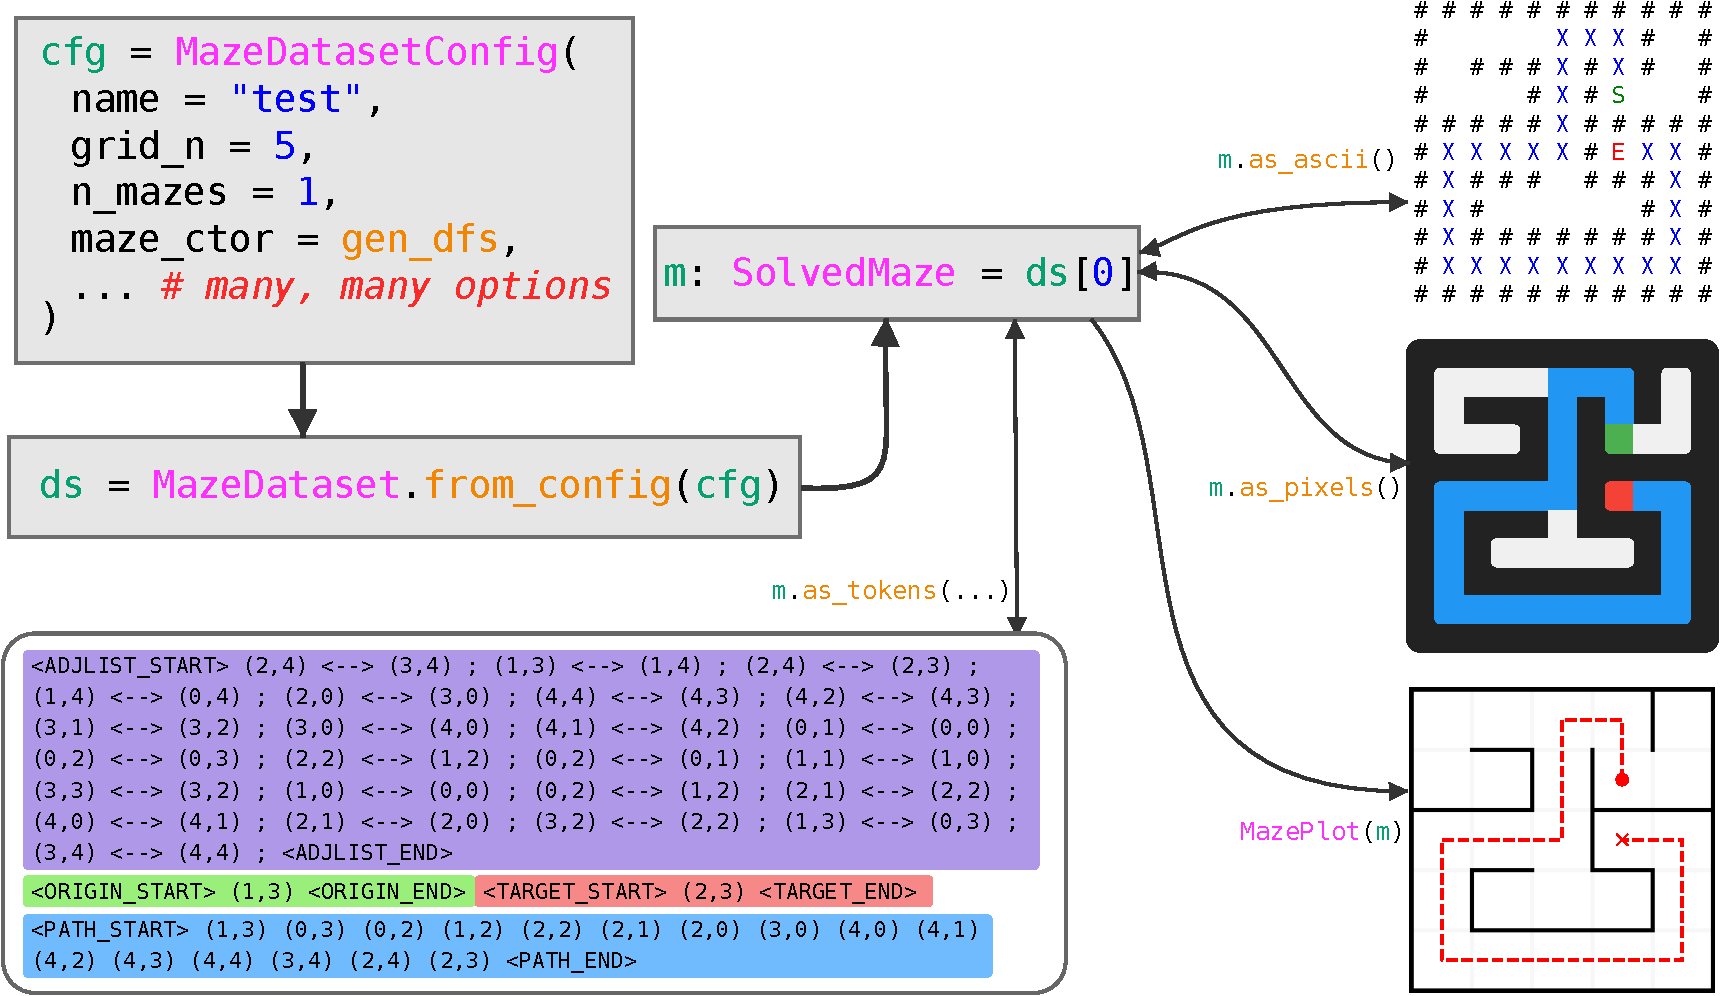
\includegraphics{docs/paper/diagram/diagram.pdf}%
};

\node[anchor=north west,
	hyperlink url={https://github.com},
	draw=blue, fill=blue!20, fill opacity=0.3,
	minimum width=2cm, minimum height=1cm]
	at ($(current page.north west)+(0,-1cm)$) {};

% Establish a coordinate system mapping the original SVG viewBox (1100x640)
% \begin{scope}[x={(img.south east)}, y={(img.north west)}]
	
% 	% 1. MazeDatasetConfig (for both "cfg" and "MazeDatasetConfig")
% 	\node[hyperlink url={https://understanding-search.github.io/maze-dataset/maze_dataset.html#MazeDatasetConfig},
% 			anchor=south west,
% 			draw=blue, fill=blue!20, fill opacity=0.3, line width=1pt,
% 			minimum width={(150-25)/1100*6in},
% 			minimum height={(60-30)/640*3.5in}]
% 		at ($(25/1100, {1 - 60/640})$) {};
	
% 	% 2. LatticeMazeGenerators.gen_dfs (the "gen_dfs" text)
% 	\node[hyperlink url={https://understanding-search.github.io/maze-dataset/maze_dataset.html#LatticeMazeGenerators.gen_dfs},
% 			anchor=south west,
% 			draw=blue, fill=blue!20, fill opacity=0.3, line width=1pt,
% 			minimum width={(150-45)/1100*6in},
% 			minimum height={(180-150)/640*3.5in}]
% 		at ($(45/1100, {1 - 180/640})$) {};
	
% 	% 3. MazeDataset (the "ds" and "MazeDataset" text)
% 	\node[hyperlink url={https://understanding-search.github.io/maze-dataset/maze_dataset.html#MazeDataset},
% 			anchor=south west,
% 			draw=blue, fill=blue!20, fill opacity=0.3, line width=1pt,
% 			minimum width={(150-25)/1100*6in},
% 			minimum height={(335-305)/640*3.5in}]
% 		at ($(25/1100, {1 - 335/640})$) {};
	
% 	% 4. MazeDataset.from_config (following MazeDataset on the same line)
% 	\node[hyperlink url={https://understanding-search.github.io/maze-dataset/maze_dataset.html#MazeDataset.from_config},
% 			anchor=south west,
% 			draw=blue, fill=blue!20, fill opacity=0.3, line width=1pt,
% 			minimum width={(300-150)/1100*6in},
% 			minimum height={(335-305)/640*3.5in}]
% 		at ($(150/1100, {1 - 335/640})$) {};
	
% 	% 5. SolvedMaze (the text starting at x≈424.6, y≈205)
% 	\node[hyperlink url={https://understanding-search.github.io/maze-dataset/maze_dataset.html#SolvedMaze},
% 			anchor=south west,
% 			draw=blue, fill=blue!20, fill opacity=0.3, line width=1pt,
% 			minimum width={(544.6-424.6)/1100*6in},  % 544.6 = 424.6+120
% 			minimum height={(205-165)/640*3.5in}]
% 		at ($(424.6/1100, {1 - 205/640})$) {};
	
% 	% 6. LatticeMaze.as_ascii (from x≈837.4, y≈125)
% 	\node[hyperlink url={https://understanding-search.github.io/maze-dataset/maze_dataset.html#LatticeMaze.as_ascii},
% 			anchor=south west,
% 			draw=blue, fill=blue!20, fill opacity=0.3, line width=1pt,
% 			minimum width={(937.4-837.4)/1100*6in},  % 937.4 = 837.4+100
% 			minimum height={(125-95)/640*3.5in}]
% 		at ($(837.4/1100, {1 - 125/640})$) {};
	
% 	% 7. LatticeMaze.as_pixels (from x≈836.1, y≈335)
% 	\node[hyperlink url={https://understanding-search.github.io/maze-dataset/maze_dataset.html#LatticeMaze.as_pixels},
% 			anchor=south west,
% 			draw=blue, fill=blue!20, fill opacity=0.3, line width=1pt,
% 			minimum width={(936.1-836.1)/1100*6in},  % 936.1 = 836.1+100
% 			minimum height={(335-305)/640*3.5in}]
% 		at ($(836.1/1100, {1 - 335/640})$) {};
	
% 	% 8. MazePlot (from x≈846.8, y≈555)
% 	\node[hyperlink url={https://understanding-search.github.io/maze-dataset/maze_dataset/plotting.html#MazePlot},
% 			anchor=south west,
% 			draw=blue, fill=blue!20, fill opacity=0.3, line width=1pt,
% 			minimum width={(966.8-846.8)/1100*6in},  % 966.8 = 846.8+120
% 			minimum height={(555-525)/640*3.5in}]
% 		at ($(846.8/1100, {1 - 555/640})$) {};
	
% 	% 9. LatticeMaze.as_tokens (from x≈571.1, y≈406)
% 	\node[hyperlink url={https://understanding-search.github.io/maze-dataset/maze_dataset.html#LatticeMaze.as_tokens},
% 			anchor=south west,
% 			draw=blue, fill=blue!20, fill opacity=0.3, line width=1pt,
% 			minimum width={(691.1-571.1)/1100*6in},  % 691.1 = 571.1+120
% 			minimum height={(406-376)/640*3.5in}]
% 		at ($(571.1/1100, {1 - 406/640})$) {};
	
% \end{scope}
\end{tikzpicture} 
	\end{minipage}
	\caption{
	  Usage of maze-dataset. We create a \texttt{MazeDataset} from a \texttt{MazeDatasetConfig}. This contains \texttt{SolvedMaze} objects which can be converted to and from a variety of formats. Code in the image contains clickable links to \docslink{maze_dataset.html}{documentation}. A variety of generated examples can be viewed \docslink{examples/maze_examples.html}{here}.
	}
	\label{fig:diagram}
\end{figure}

\section{Statement of Need}\label{statement-of-need}

While maze generation itself is straightforward, the architectural
challenge comes from building a system supporting many algorithms with
configurable parameters, property filtering, and representation
transformation. This library aims to greatly streamline the process of
generating and working with datasets of mazes that can be described as
subgraphs of an \(n \times n\) lattice with boolean connections and,
optionally, start and end points that are nodes in the graph.
Furthermore, we place emphasis on a wide variety of possible text output
formats aimed at evaluating the spatial reasoning capabilities of Large
Language Models (LLMs) and other text-based transformer models.

For interpretability and behavioral research, algorithmic tasks offer
benefits by allowing systematic data generation and task decomposition,
as well as simplifying the process of circuit discovery
(\citeproc{ref-interpretability-survey}{Räuker et al., 2023}). Although
mazes are well suited for these investigations, we found that existing
maze generation packages (\citeproc{ref-cobbe2019procgen}{Cobbe et al.,
2019}; \citeproc{ref-gh_Ehsan_2022}{Ehsan, 2022};
\citeproc{ref-harriesMazeExplorerCustomisable3D2019}{Harries et al.,
n.d.}; \citeproc{ref-gh_Nemeth_2019}{Németh, 2019};
\citeproc{ref-easy_to_hard}{Schwarzschild, Borgnia, Gupta, Bansal, et
al., 2021}) lack support for transforming between multiple
representations and provide limited control over the maze generation
process.

\subsection{Related Works}\label{related-works}

A multitude of public and open-source software packages exist for
generating mazes (\citeproc{ref-gh_Ehsan_2022}{Ehsan, 2022};
\citeproc{ref-gh_Nemeth_2019}{Németh, 2019};
\citeproc{ref-easy_to_hard}{Schwarzschild, Borgnia, Gupta, Bansal, et
al., 2021}). However, nearly all of these packages produce mazes
represented as rasterized images or other visual formats rather than the
underlying graph structure, and this makes it difficult to work with
these datasets.

\begin{itemize}
\item
  Most prior works provide mazes in visual or raster formats, and we
  provide a variety of similar output formats:

  \begin{itemize}
  \tightlist
  \item
    \href{https://understanding-search.github.io/maze-dataset/maze_dataset/dataset/rasterized.html\#RasterizedMazeDataset}{\texttt{RasterizedMazeDataset}},
    utilizing
    \href{https://understanding-search.github.io/maze-dataset/maze_dataset.html\#LatticeMaze.as_pixels}{\texttt{as\_pixels()}},
    which can exactly mimic the outputs provided in
    \texttt{easy-to-hard-data}
    (\citeproc{ref-easy_to_hard}{Schwarzschild, Borgnia, Gupta, Bansal,
    et al., 2021}) and can be configured to be similar to the outputs of
    Németh (\citeproc{ref-gh_Nemeth_2019}{2019})
  \item
    \href{https://understanding-search.github.io/maze-dataset/maze_dataset.html\#LatticeMaze.as_ascii}{\texttt{as\_ascii()}}
    provides a format similar to
    (\citeproc{ref-gh-oppenheimj2018maze}{Oppenheim, 2018};
    \citeproc{ref-eval-gpt-visual}{Singla, 2023})
  \item
    \href{https://understanding-search.github.io/maze-dataset/maze_dataset/plotting.html\#MazePlot}{\texttt{MazePlot}}
    provides a feature‑rich plotting utility with support for multiple
    paths, heatmaps over positions, and more. This is similar to the
    outputs of (\citeproc{ref-mazegenerator-net}{Alance AB, 2019};
    \citeproc{ref-gh_Ehsan_2022}{Ehsan, 2022};
    \citeproc{ref-mathematica-maze}{Guo et al., 2011};
    \citeproc{ref-mdl-suite}{Nag, 2020})
  \end{itemize}
\item
  The text format provided by
  \href{https://understanding-search.github.io/maze-dataset/maze_dataset.html\#MazeDataset.as_tokens}{\texttt{SolvedMaze(...).as\_tokens()}}
  is similar to that of (\citeproc{ref-eval-LLM-graphs}{Liu \& Wu,
  2023}) but with many more options, detailed in
  \hyperref[sec:tokenized-output-formats]{section: \textit{\nameref{sec:tokenized-output-formats}}}.
\item
  Preserving metadata about the generation algorithm with the dataset
  itself is essential for studying the effects of distributional shifts.
  Our package efficiently stores the dataset along with its metadata in
  a single human-readable file (\citeproc{ref-zanj}{M. Ivanitskiy,
  n.d.}). As far as we are aware, no existing packages do this reliably.
\item
  Storing mazes as images or adjacency matrices is not only difficult to
  work with, but also inefficient. We use a highly efficient method
  detailed in
  \hyperref[sec:implementation]{section: \textit{\nameref{sec:implementation}}}.
\item
  Our package is easily installable with source code freely available.
  It is extensively tested, type hinted, benchmarked, and documented.
  Many other maze generation packages lack this level of rigor and
  scope, and some (\citeproc{ref-ayaz2008maze}{Ayaz et al., 2008})
  appear to simply no longer be accessible.
\end{itemize}

\newpage

\section{Features}\label{features}

We direct readers to our
\href{https://understanding-search.github.io/maze-dataset/examples/maze_examples.html}{examples},
\href{https://understanding-search.github.io/maze-dataset/maze_dataset.html}{docs},
and
\href{https://understanding-search.github.io/maze-dataset/notebooks/}{notebooks}
for more information. Our package can be installed from
\href{https://pypi.org/project/maze-dataset/}{PyPi} via
\texttt{pip\ install\ maze-dataset}, or directly from the
\href{https://github.com/understanding-search/maze-dataset}{git
repository} (\citeproc{ref-maze-dataset-github}{Michael I. Ivanitskiy et
al., 2023a}).

Datasets of mazes are created from a
\href{https://understanding-search.github.io/maze-dataset/maze_dataset.html\#MazeDatasetConfig}{\texttt{MazeDatasetConfig}}
configuration object, which allows specifying the number of mazes, their
size, the generation algorithm, and various parameters for the
generation algorithm. Datasets can also be filtered after generation to
satisfy certain properties. Custom filters can be specified, and some
filters are included in
\href{https://understanding-search.github.io/maze-dataset/maze_dataset/dataset/filters.html\#MazeDatasetFilters}{\texttt{MazeDatasetFilters}}.

\subsection{Visual Output Formats}\label{visual-output-formats}

Internally, mazes are
\href{https://understanding-search.github.io/maze-dataset/maze_dataset.html\#SolvedMaze}{\texttt{SolvedMaze}}
objects, which have path information and a tensor optimized for storing
sub-graphs of a lattice. These objects can be converted to and from
several formats, shown in \autoref{fig:output-fmts}, to maximize their
utility in different contexts.

In previous work, maze tasks have been used with Recurrent Convolutional
Neural Network (RCNN) derived architectures
(\citeproc{ref-deepthinking}{Schwarzschild, Borgnia, Gupta, Huang, et
al., 2021}). To facilitate the use of our package in this context, we
replicate the format of (\citeproc{ref-easy_to_hard}{Schwarzschild,
Borgnia, Gupta, Bansal, et al., 2021}) and provide the
\href{https://understanding-search.github.io/maze-dataset/maze_dataset/dataset/rasterized.html\#RasterizedMazeDataset}{\texttt{RasterizedMazeDataset}}
class which returns rasterized pairs of (input, target) mazes as shown
in \autoref{fig:e2h-raster}.

\begin{figure}[H]
	\centering
	\begin{tabular}{p{1.5in} p{1.5in} p{1.5in}} 
	  \hline \\[.5em]
	  % algorithms
	  \docslink{maze_dataset.html\#LatticeMaze.as_ascii}{\texttt{as\_ascii()}}
	  & \docslink{maze_dataset.html\#LatticeMaze.as_pixels}{\texttt{as\_pixels()}}
	  & \docslink{maze_dataset/plotting.html\#MazePlot}{\texttt{MazePlot()}} \\[.5em]
	  % descriptions
		Simple text format for displaying mazes, useful for debugging in a terminal environment.
		& \texttt{numpy} array of \texttt{dtype=uint8} and shape \texttt{(height, width, 3)}. The last dimension is RGB color.
		& feature-rich plotting utility with support for multiple paths, heatmaps over positions, and more. \\[1em]
	  \hline \\
	  % examples
		\multicolumn{1}{l}{
		  \hspace{-1.5em}\raisebox{0.85\height}{
			  {
% \footnotesize
\ttfamily
\setlength{\tabcolsep}{0.3em}
\renewcommand{\arraystretch}{0.75}
\begin{tabular}{ccccccccccc}
\# & \# & \# & \# & \# & \# & \# & \# & \# & \# & \# \\
\# &   &   &   &   & \textcolor{blue}{X} & \textcolor{blue}{X} & \textcolor{blue}{X} & \# &  & \# \\
\# &   & \# & \# & \# & \textcolor{blue}{X} & \# & \textcolor{blue}{X} & \# &   & \# \\
\# &   &   &   & \# & \textcolor{blue}{X} & \# & \textcolor{green}{S} &   &   & \# \\
\# & \# & \# & \# & \# & \textcolor{b			lue}{X} & \# & \# & \# & \# & \# \\
\# & \textcolor{blue}{X} & \textcolor{blue}{X} & \textcolor{blue}{X} & \textcolor{blue}{X} & \textcolor{blue}{X} & \# & \textcolor{red}{E} & \textcolor{blue}{X} & \textcolor{blue}{X} & \# \\
\# & \textcolor{blue}{X} & \# & \# & \# &   & \# & \# & \# & \textcolor{blue}{X} & \# \\
\# & \textcolor{blue}{X} & \# &   &   &   &   &   & \# & \textcolor{blue}{X} & \# \\
\# & \textcolor{blue}{X} & \# & \# & \# & \# & \# & \# & \# & \textcolor{blue}{X} & \# \\
\# & \textcolor{blue}{X} & \textcolor{blue}{X} & \textcolor{blue}{X} & \textcolor{blue}{X} & \textcolor{blue}{X} & \textcolor{blue}{X} & \textcolor{blue}{X} & \textcolor{blue}{X} & \textcolor{blue}{X} & \# \\
\# & \# & \# & \# & \# & \# & \# & \# & \# & \# & \#
\end{tabular}
}
		  }
		}
		% 	\begin{minipage}[b]{1.6in}
		%   \setlength{\baselineskip}{0.9em}
		% 	\end{minipage}
		& \multicolumn{1}{c}{
		  
\includegraphics[width=0.25\textwidth]{figures/outputs-pixels.pdf}
		}
		& \multicolumn{1}{r}{
		  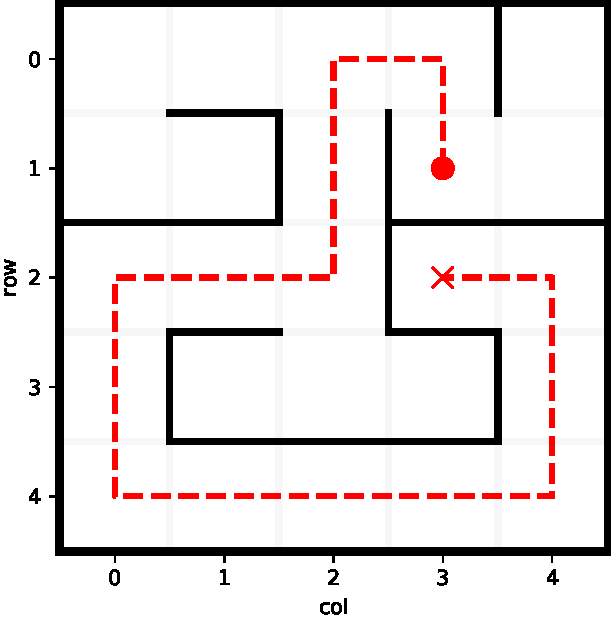
\includegraphics[width=0.27\textwidth, trim={0 0.8cm -.3cm, -.5cm}, clip]{figures/outputs-mazeplot.pdf}
		} \\[1em]
	  
	  \hline \\
	\end{tabular}
	\caption{Various output formats. Top row (left to right): ASCII diagram, rasterized pixel grid, and advanced display tool.}
	\label{fig:output-fmts}
\end{figure}

\begin{figure}
	\centering
	
\includegraphics[width=0.3\textwidth]{figures/maze-raster-input-target.pdf}
	\caption{
		Input is the rasterized maze without the path marked (left), and provide as a target the maze with all but the correct path removed (right). Configuration options exist to adjust whether endpoints are included and if empty cells should be filled in.
	}
	\label{fig:e2h-raster}
\end{figure}

\newpage

\subsection{Tokenized Output
Formats}\label{sec:tokenized-output-formats}

Autoregressive transformer models can be quite sensitive to the exact
format of input data, and may even use delimiter tokens to perform
reasoning steps (\citeproc{ref-pfau2024dotbydot}{Pfau et al., 2024};
\citeproc{ref-spies2024causalworldmodels}{Spies et al., 2024}). To
facilitate systematic investigation of the effects of different
representations of data on text model performance, we provide a variety
of text output formats, with an example given in
\autoref{fig:token-regions}. We utilize Finite State Transducers
(\citeproc{ref-Gallant2015Transducers}{Gallant, 2015}) for efficiently
storing valid tokenizers.

\begin{figure} 
	\centering
	\begin{minipage}{5in}
	  \footnotesize
	  % could not figure out how to make lines break a colorbox, so that's why these line breaks are manual
\colorbox[RGB]{ 217,210,233 }{ \texttt{ <ADJLIST\_START> (0,0) <--> (1,0) ; (2,0) <--> (3,0) ; (4,1) <--> (4,0) ; (2,0) <--> (2,1) ; }} 
\colorbox[RGB]{ 217,210,233 }{ \texttt{ (1,0) <--> (1,1) ; (3,4) <--> (2,4) ; (4,2) <--> (4,3) ; (0,0) <--> (0,1) ; (0,3) <--> (0,2) ; }}
\colorbox[RGB]{ 217,210,233 }{ \texttt{ (4,4) <--> (3,4) ; (4,3) <--> (4,4) ; (4,1) <--> (4,2) ; (2,1) <--> (2,2) ; (1,4) <--> (0,4) ; }}
\colorbox[RGB]{ 217,210,233 }{ \texttt{ (1,2) <--> (0,2) ; (2,4) <--> (2,3) ; (4,0) <--> (3,0) ; (2,2) <--> (3,2) ; (1,2) <--> (2,2) ; }} 
\colorbox[RGB]{ 217,210,233 }{ \texttt{ (1,3) <--> (0,3) ; (3,2) <--> (3,3) ; (0,2) <--> (0,1) ; (3,1) <--> (3,2) ; (1,3) <--> (1,4) ; }}
\colorbox[RGB]{ 217,210,233 }{ \texttt{ <ADJLIST\_END> } } \colorbox[RGB]{ 217,234,211 }{ \texttt{ <ORIGIN\_START> (1,3) <ORIGIN\_END> } } 
\colorbox[RGB]{ 234,209,220 }{ \texttt{ <TARGET\_START> (2,3) <TARGET\_END> } } 
\colorbox[RGB]{ 207,226,243 }{ \texttt{ <PATH\_START> (1,3) (0,3) (0,2) (1,2) (2,2) (2,1) (2,0) (3,0) (4,0) (4,1) (4,2) (4,3) (4,4) }}
\colorbox[RGB]{ 207,226,243 }{ \texttt{ (3,4) (2,4) (2,3) <PATH\_END> } } \\
	\end{minipage}
	\caption{
	  Example text output format with token regions highlighted.
	  \colorbox[RGB]{ 217,210,233 }{Adjacency list}: text representation of the graph,
	  \colorbox[RGB]{ 217,234,211 }{Origin}: starting coordinate,
	  \colorbox[RGB]{ 234,209,220 }{Target}: ending coordinate,
	  \colorbox[RGB]{ 207,226,243 }{Path}: maze solution sequence
	}
	\label{fig:token-regions}
\end{figure}

\subsection{Benchmarks}\label{benchmarks}

We benchmarks for generation time across various configurations in
\autoref{tab:benchmarks} and \autoref{fig:benchmarks}. Experiments were
performed on a
\href{https://docs.github.com/en/actions/using-github-hosted-runners/using-github-hosted-runners/about-github-hosted-runners\#standard-github-hosted-runners-for-public-repositories}{standard
GitHub runner} without parallelism. Additionally, maze generation under
certain constraints may not always be successful, and for this we
provide a way to estimate the success rate of a given configuration,
described in \autoref{fig:sre}.

\begin{table}[H]
\centering
\begin{tabular}{|ll|r|rrr|}
	\hline
	maze\_ctor
			& keyword args           & all sizes 
												& \shortstack{small \\ $g \leq 10$} 
															& \shortstack{medium \\ $g \in (10, 32]$} 
																	& \shortstack{large \\ $g > 32$} \\
	\hline\hline
	\docslink{maze_dataset.html\#LatticeMazeGenerators.gen_dfs}{dfs}
			&                        &   28.0   &    2.8   &   20.3   &  131.8   \\
	\docslink{maze_dataset.html\#LatticeMazeGenerators.gen_dfs}{dfs}
			& accessible\_cells=20   &    2.3   &    2.2   &    2.4   &    2.2   \\
	\docslink{maze_dataset.html\#LatticeMazeGenerators.gen_dfs}{dfs}
			& do\_forks=False        &    2.7   &    2.2   &    3.1   &    3.5   \\
	\docslink{maze_dataset.html\#LatticeMazeGenerators.gen_dfs}{dfs}
			& max\_tree\_depth=0.5   &    2.5   &    2.0   &    2.7   &    4.0   \\
	\docslink{maze_dataset.html\#LatticeMazeGenerators.gen_dfs_percolation}{dfs\_percolation}
			& p=0.1                  &   43.9   &    2.8   &   33.9   &  208.0   \\
	\docslink{maze_dataset.html\#LatticeMazeGenerators.gen_dfs_percolation}{dfs\_percolation}
			& p=0.4                  &   48.7   &    3.0   &   36.5   &  233.5   \\
	\docslink{maze_dataset.html\#LatticeMazeGenerators.gen_kruskal}{kruskal}
			&                        &   12.8   &    1.9   &   10.3   &   55.8   \\
	\docslink{maze_dataset.html\#LatticeMazeGenerators.gen_percolation}{percolation}
			& p=1.0                  &   50.2   &    2.6   &   37.2   &  242.5   \\
	\docslink{maze_dataset.html\#LatticeMazeGenerators.gen_recursive_division}{recursive\_div}
			&                        &   10.2   &    1.7   &    8.9   &   42.1   \\
	\docslink{maze_dataset.html\#LatticeMazeGenerators.gen_wilson}{wilson}
			&                        &  676.5   &    7.8   &  188.6   & 3992.6   \\
	\hline\hline
	mean
			&                        &  559.9   &   13.0   &  223.5   & 3146.9   \\
	median
			&                        &   11.1   &    6.5   &   32.9   &  302.7   \\
	\hline
\end{tabular}
\caption{Generation times in milliseconds for various algorithms and maze sizes. More information can be found on the \docslink{benchmarks}{benchmarks page}.}
\label{tab:benchmarks}
\end{table}

\begin{figure}
	\hypertarget{fig:benchmarks}{%
		\centering
		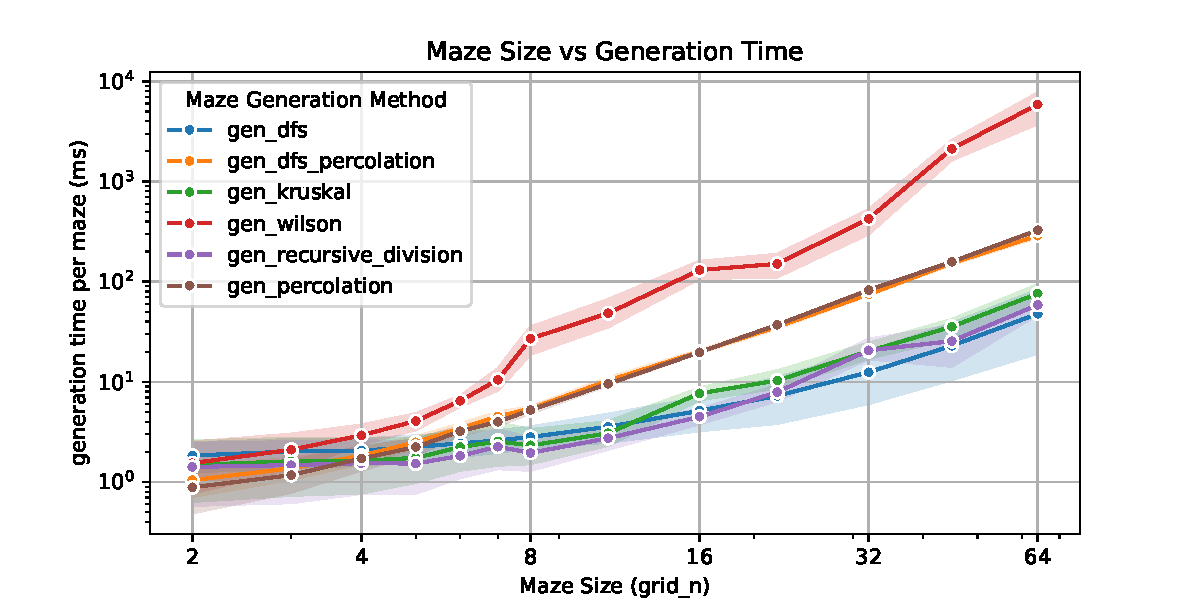
\includegraphics[width=\textwidth]{figures/benchmarks/gridsize-vs-gentime.pdf}
		\caption{
			Plot of maze generation time. Generation time scales
			exponentially with maze size for all algorithms. Generation time per
			maze does not depend on the number of mazes being generated, and there
			is minimal overhead to initializing the generation process for a small
			dataset. Wilson's algorithm is notably less efficient than others and
			has high variance. Note that values are averaged across all parameter
			sets for that algorithm. More information can be found on the
			\href{https://understanding-search.github.io/maze-dataset/benchmarks/}{benchmarks page}.
		}
		\label{fig:benchmarks}
	}
\end{figure}

\begin{figure}
	\centering
	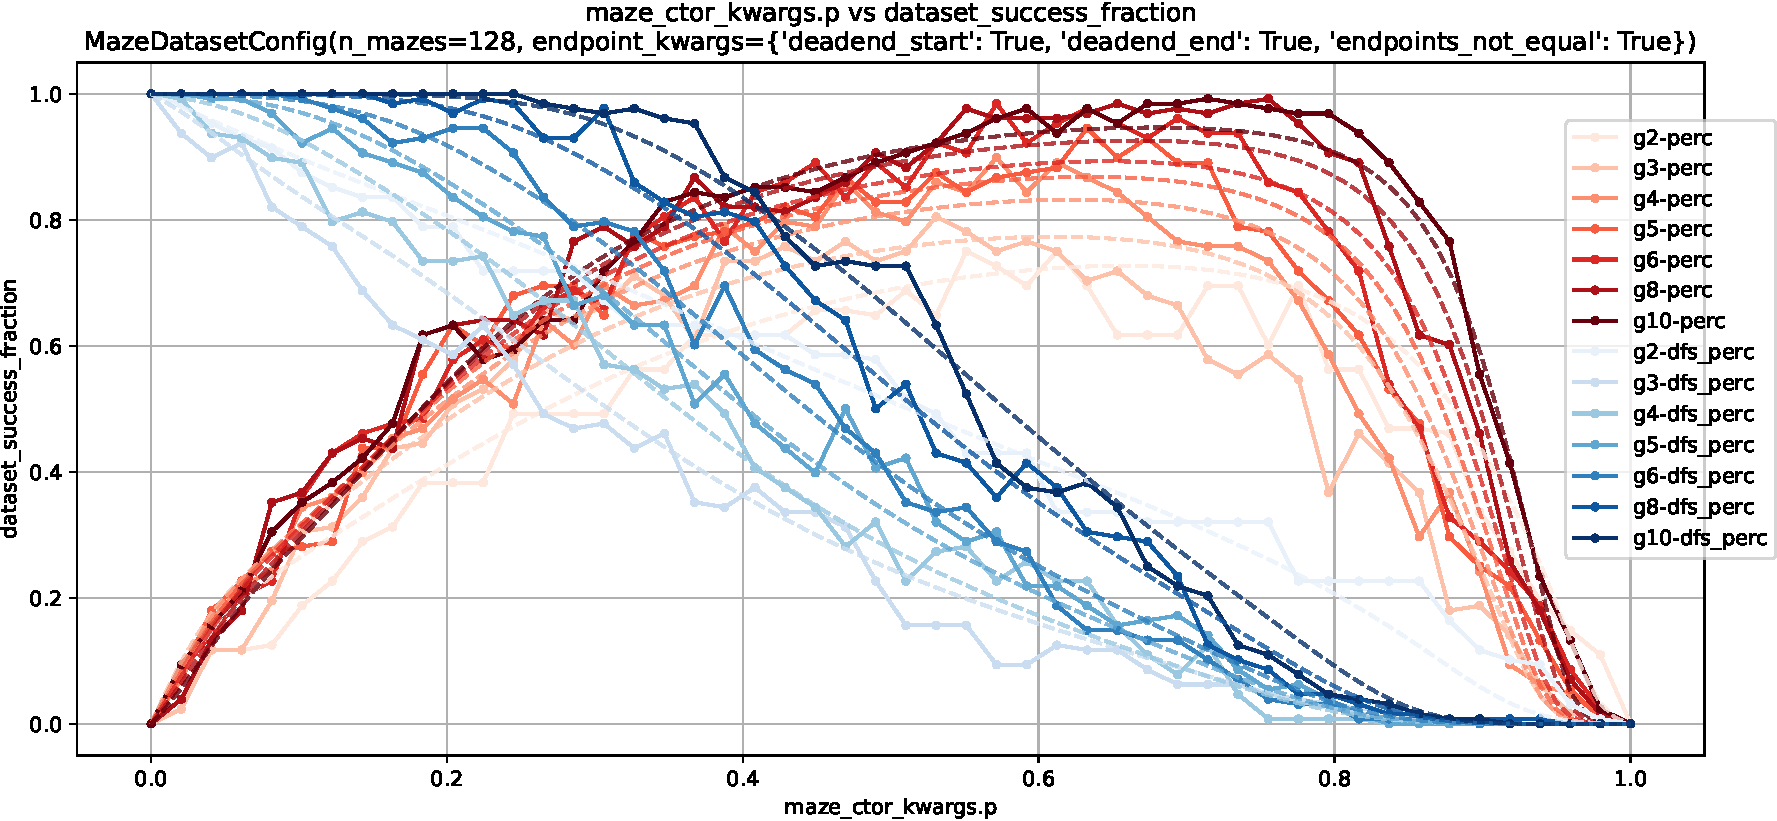
\includegraphics[width=1\textwidth,height=\textheight]{figures/ep/ep_deadends_unique-crop.pdf}
	\caption{
		In order to replicate the exact dataset distribution of \cite{easy_to_hard}, the parameter \href{https://understanding-search.github.io/maze-dataset/maze_dataset/dataset/maze_dataset_config.html#MazeDatasetConfig.endpoint_kwargs}{\texttt{MazeDatasetConfig.endpoint\_kwargs}} allows for additional constraints, such as enforcing that the start or end point be in a ``dead end'' with only one accessible neighbor cell. However, combining these constraints with cyclic mazes can lead to an absence of valid start and end points. To deal with this, our package provides a way to estimate the success rate of a given configuration using a symbolic regression model trained with PySR \cite{pysr}.
		An example of both empirical and predicted success rates as a function of the percolation probability \(p\) for various maze sizes, percolation with and without depth first search, and \texttt{endpoint\_kwargs} requiring that both the start and end be in unique dead ends. Empirical measures derived from a sample of 128 mazes. More information can be found on the \href{https://understanding-search.github.io/maze-dataset/benchmarks/}{benchmarks page} and in the notebook \href{https://understanding-search.github.io/maze-dataset/notebooks/estimate_dataset_fractions.html}{\texttt{estimate\_dataset\_fractions.ipynb}}.
	}
	\label{fig:sre}
\end{figure}

\section{Implementation}\label{sec:implementation}

Using an adjacency matrix for storing mazes would be memory inefficient
by failing to exploit the highly sparse structure, while using an
adjacency list could lead to a poor lookup time. This package utilizes a
simple, efficient representation of mazes as subgraphs of a finite
lattice, detailed in \autoref{fig:maze-impl}, which we call a
\href{https://understanding-search.github.io/maze-dataset/maze_dataset.html\#LatticeMaze}{\texttt{LatticeMaze}}.

\begin{figure}
\centering
\begin{tabular}{ccc}
	Maze 
	& $A[0]$ (downward)
	& $A[1]$ (rightward) \\
	\raisebox{-0.5\height}{
		
\includegraphics[width=5em]{figures/tex/maze-impl.pdf}
	}
	& \raisebox{-0.5em}{
		\large $\begin{bmatrix}
			1 & 1 & 1 \\
			0 & 0 & 1 \\
			0 & 0 & 0
		\end{bmatrix}$
	}
	& \raisebox{-0.5em}{
		\large $\begin{bmatrix}
			1 & 0 & 0 \\
			0 & 1 & 0 \\
			1 & 1 & 0
		\end{bmatrix}$
	}
\end{tabular}
\caption{
	We describe mazes with the following representation: for a $2$-dimensional lattice with $r$ rows and $c$ columns, we initialize a boolean array $A = \{0, 1\}^{2 \times r \times c}$ which we refer to in the code as a \href{https://understanding-search.github.io/maze-dataset/maze_dataset.html#LatticeMaze.connection_list}{\texttt{connection\_list}}. The value at $A[0,i,j]$ determines whether a \emph{downward} connection exists from node $[i,j]$ to $[i+1, j]$. Likewise, the value at $A[1,i,j]$ determines whether a \emph{rightward} connection to $[i, j+1]$ exists. Thus, we avoid duplication of data about the existence of connections and facilitate fast lookup time, at the cost of requiring additional care with indexing.
}
\label{fig:maze-impl}
\end{figure}

Our package is implemented in Python(\citeproc{ref-python}{Rossum,
1995}), and makes use of the extensive scientific computing ecosystem,
including NumPy (\citeproc{ref-numpy}{Harris et al., 2020}) for array
manipulation, plotting tools (\citeproc{ref-matplotlib}{Hunter, 2007};
\citeproc{ref-seaborn}{Waskom, 2021}), Jupyter notebooks
(\citeproc{ref-jupyter}{Kluyver et al., 2016}), and PySR
(\citeproc{ref-pysr}{Cranmer, 2023}) for symbolic regression.

\section{Usage in Research}\label{usage-in-research}

This package was originally built for the needs of the
(\citeproc{ref-maze-transformer-github}{Michael I. Ivanitskiy et al.,
2023b}) project, which aims to investigate spatial planning and world
models in autoregressive transformer models trained on mazes
(\citeproc{ref-ivanitskiy2023structuredworldreps}{Michael Igorevich
Ivanitskiy, Spies, et al., 2023};
\citeproc{ref-maze-dataset-arxiv-2023}{Michael Igorevich Ivanitskiy,
Shah, et al., 2023}; \citeproc{ref-spies2024causalworldmodels}{Spies et
al., 2024}). It was extended for work on understanding the mechanisms by
which recurrent convolutional and implicit networks
(\citeproc{ref-fung2022jfb}{Fung et al., 2022}) solve mazes given a
rasterized view (\citeproc{ref-knutson2024logicalextrapolation}{Knutson
et al., 2024}), which required matching the pixel-padded and endpoint
constrained output format of (\citeproc{ref-easy_to_hard}{Schwarzschild,
Borgnia, Gupta, Bansal, et al., 2021}). Ongoing work using
\texttt{maze-dataset} aims to investigate the effects of varying the
tokenization format on the performance of pretrained LLMs on spatial
reasoning.

This package has also been utilized in work by other groups:

\begin{itemize}
\item
  By (\citeproc{ref-nolte2024multistep}{Nolte et al., 2024}) to compare
  the effectiveness of transformers trained with the MLM-\(\mathcal{U}\)
  (\citeproc{ref-MLMU-kitouni2024factorization}{Kitouni et al., 2024})
  multistep prediction objective against standard autoregressive
  training for multi-step planning on our maze task.
\item
  By (\citeproc{ref-wang2024imperative}{Wang et al., 2024}) and
  (\citeproc{ref-chen2024iaimperative}{Chen et al., 2024}) to study the
  effectiveness of imperative learning.
\item
  By (\citeproc{ref-zhang2025tscend}{Zhang et al., 2025}) to introduce a
  novel framework for reasoning diffusion models.
\item
  By (\citeproc{ref-dao2025alphamaze}{Dao \& Vu, 2025}) to improve
  spatial reasoning in LLMs with GRPO.
\end{itemize}

\section{Acknowledgements}\label{acknowledgements}

This work was partially funded by National Science Foundation awards DMS-2110745 and DMS-2309810. We are also grateful to LTFF and FAR Labs for hosting authors MII, AFS, and TR for a residency visit, and to various members of FAR's technical staff for their advice.

This work was partially supported by AI Safety Camp and AI Safety Support, which also brought many of the authors together. We would like to thank our former collaborators at AI Safety Camp and other users and contributors to the  \texttt{maze-dataset} package: Benji Berczi, Guillaume Corlouer, William Edwards, Leon Eshuijs, Chris Mathwin, Lucia Quirke, Can Rager, Adrians Skapars, Rusheb Shah, Johannes Treutlein, and Dan Valentine.

We thank the Mines Optimization and Deep Learning group (MODL) for fruitful discussions. We also thank Michael Rosenberg for recommending the usage of Finite State Transducers for storing tokenizer validation information.

\newpage

\section*{References}\label{references}
\addcontentsline{toc}{section}{References}

\phantomsection\label{refs}
\begin{CSLReferences}{1}{0.5}
\bibitem[\citeproctext]{ref-mazegenerator-net}
Alance AB. (2019). \emph{Maze generator}.
\url{http://www.mazegenerator.net}.

\bibitem[\citeproctext]{ref-ayaz2008maze}
Ayaz, H., Allen, S. L., Platek, S. M., \& Onaral, B. (2008). Maze suite
1.0: A complete set of tools to prepare, present, and analyze
navigational and spatial cognitive neuroscience experiments.
\emph{Behavior Research Methods}, \emph{40}, 353--359.
\url{https://doi.org/10.3758/brm.40.1.353}

\bibitem[\citeproctext]{ref-chen2024iaimperative}
Chen, X., Yang, F., \& Wang, C. (2024). {iA*}: Imperative learning-based
{A*} search for pathfinding. \emph{arXiv Preprint arXiv:2403.15870}.
\url{https://doi.org/10.48550/arXiv.2403.15870}

\bibitem[\citeproctext]{ref-cobbe2019procgen}
Cobbe, K., Hesse, C., Hilton, J., \& Schulman, J. (2019). Leveraging
procedural generation to benchmark reinforcement learning. \emph{arXiv
Preprint arXiv:1912.01588}.
\url{https://doi.org/10.48550/arXiv.1912.01588}

\bibitem[\citeproctext]{ref-pysr}
Cranmer, M. (2023). Interpretable machine learning for science with PySR
and SymbolicRegression. jl. \emph{arXiv Preprint arXiv:2305.01582}.
\url{https://doi.org/10.48550/arXiv.2305.01582}

\bibitem[\citeproctext]{ref-dao2025alphamaze}
Dao, A., \& Vu, D. B. (2025). AlphaMaze: Enhancing large language
models' spatial intelligence via GRPO. \emph{arXiv Preprint
arXiv:2502.14669}. \url{https://doi.org/10.48550/arXiv.2502.14669}

\bibitem[\citeproctext]{ref-gh_Ehsan_2022}
Ehsan, E. (2022). \emph{Maze}. \url{https://github.com/emadehsan/maze}

\bibitem[\citeproctext]{ref-fung2022jfb}
Fung, S. W., Heaton, H., Li, Q., McKenzie, D., Osher, S., \& Yin, W.
(2022). Jfb: Jacobian-free backpropagation for implicit networks.
\emph{Proceedings of the AAAI Conference on Artificial Intelligence},
\emph{36}, 6648--6656. \url{https://doi.org/10.1609/aaai.v36i6.20619}

\bibitem[\citeproctext]{ref-Gallant2015Transducers}
Gallant, A. (2015). \emph{Index 1,600,000,000 keys with automata and
rust}. \url{https://burntsushi.net/transducers/}.

\bibitem[\citeproctext]{ref-mathematica-maze}
Guo, C., Barthelet, L., \& Morris, R. (2011). \emph{Maze generator and
solver}. Wolfram Demonstrations Project,
\url{https://demonstrations.wolfram.com/MazeGeneratorAndSolver/}.

\bibitem[\citeproctext]{ref-harriesMazeExplorerCustomisable3D2019}
Harries, L., Lee, S., Rzepecki, J., Hofmann, K., \& Devlin, S. (n.d.).
{MazeExplorer}: {A Customisable 3D Benchmark} for {Assessing
Generalisation} in {Reinforcement Learning}. \emph{2019 {IEEE Conf}.
{Games CoG}}, 1--4. \url{https://doi.org/10.1109/cig.2019.8848048}

\bibitem[\citeproctext]{ref-numpy}
Harris, C. R., Millman, K. J., Walt, S. J. van der, Gommers, R.,
Virtanen, P., \& al., et. (2020). Array programming with NumPy.
\emph{Nature}, \emph{585}, 357--362.
\url{https://doi.org/10.1038/s41586-020-2649-2}

\bibitem[\citeproctext]{ref-matplotlib}
Hunter, J. D. (2007). Matplotlib: A 2D graphics environment.
\emph{Computing in Science and Engineering}, \emph{9}(3), 90--95.
\url{https://doi.org/10.1109/MCSE.2007.55}

\bibitem[\citeproctext]{ref-zanj}
Ivanitskiy, M. (n.d.). \emph{ZANJ}.
\url{https://doi.org/10.5281/zenodo.15540393}

\bibitem[\citeproctext]{ref-maze-dataset-github}
Ivanitskiy, Michael I., Shah, R., Spies, A. F., Räuker, T., Valentine,
D., Rager, C., Quirke, L., Corlouer, G., \& Mathwin, C. (2023a).
\emph{Maze dataset}. \url{https://doi.org/10.48550/arXiv.2309.10498}

\bibitem[\citeproctext]{ref-maze-transformer-github}
Ivanitskiy, Michael I., Shah, R., Spies, A. F., Räuker, T., Valentine,
D., Rager, C., Quirke, L., Corlouer, G., \& Mathwin, C. (2023b).
\emph{Maze transformer interpretability}.
\url{https://doi.org/10.48550/arXiv.2312.02566}

\bibitem[\citeproctext]{ref-maze-dataset-arxiv-2023}
Ivanitskiy, Michael Igorevich, Shah, R., Spies, A. F., Räuker, T.,
Valentine, D., Rager, C., Quirke, L., Mathwin, C., Corlouer, G., Behn,
C. D., \& others. (2023). A configurable library for generating and
manipulating maze datasets. \emph{arXiv Preprint arXiv:2309.10498}.
\url{https://doi.org/10.48550/arXiv.2309.10498}

\bibitem[\citeproctext]{ref-ivanitskiy2023structuredworldreps}
Ivanitskiy, Michael Igorevich, Spies, A. F., Räuker, T., Corlouer, G.,
Mathwin, C., Quirke, L., Rager, C., Shah, R., Valentine, D., Behn, C.
D., \& others. (2023). Structured world representations in maze-solving
transformers. \emph{arXiv Preprint arXiv:2312.02566}.
\url{https://doi.org/10.48550/arXiv.2312.02566}

\bibitem[\citeproctext]{ref-MLMU-kitouni2024factorization}
Kitouni, O., Nolte, N. S., Williams, A., Rabbat, M., Bouchacourt, D., \&
Ibrahim, M. (2024). The factorization curse: Which tokens you predict
underlie the reversal curse and more. \emph{Advances in Neural
Information Processing Systems}, \emph{37}, 112329--112355.
\url{https://doi.org/10.48550/arXiv.2406.05183}

\bibitem[\citeproctext]{ref-jupyter}
Kluyver, T., Ragan-Kelley, B., Perez, F., Granger, B., Bussonnier, M.,
Frederic, J., Kelley, K., Hamrick, J., Grout, J., Corlay, S., Ivanov,
P., Avila, D., Abdalla, S., \& Willing, C. (2016). Jupyter notebooks - a
publishing format for reproducible computational workflows.
\emph{Proceedings of the 20th International Conference on Electronic
Publishing}, 87--90. \url{https://doi.org/10.3233/978-1-61499-649-1-87}

\bibitem[\citeproctext]{ref-knutson2024logicalextrapolation}
Knutson, B., Rabeendran, A. C., Ivanitskiy, M., Pettyjohn, J.,
Diniz-Behn, C., Fung, S. W., \& McKenzie, D. (2024). On logical
extrapolation for mazes with recurrent and implicit networks.
\emph{arXiv Preprint arXiv:2410.03020}.
\url{https://doi.org/10.48550/arXiv.2410.03020}

\bibitem[\citeproctext]{ref-eval-LLM-graphs}
Liu, C., \& Wu, B. (2023). Evaluating large language models on graphs:
Performance insights and comparative analysis. \emph{arXiv Preprint
arXiv:2308.11224}. \url{https://doi.org/10.48550/arXiv.2308.11224}

\bibitem[\citeproctext]{ref-mdl-suite}
Nag, A. (2020). MDL suite: A language, generator and compiler for
describing mazes. \emph{Journal of Open Source Software}, \emph{5}(46),
1815. \url{https://doi.org/10.21105/joss.01815}

\bibitem[\citeproctext]{ref-gh_Nemeth_2019}
Németh, F. (2019). \emph{Maze-generation-algorithms}.
\url{https://github.com/ferenc-nemeth/maze-generation-algorithms}

\bibitem[\citeproctext]{ref-nolte2024multistep}
Nolte, N., Kitouni, O., Williams, A., Rabbat, M., \& Ibrahim, M. (2024).
Transformers can navigate mazes with multi-step prediction. \emph{arXiv
Preprint arXiv:2412.05117}.
\url{https://doi.org/10.48550/arXiv.2412.05117}

\bibitem[\citeproctext]{ref-gh-oppenheimj2018maze}
Oppenheim, J. (2018). \emph{Maze-generator: Generate a random maze
represented as a 2D array using depth-first search}.
\url{https://github.com/oppenheimj/maze-generator/}; GitHub.

\bibitem[\citeproctext]{ref-pfau2024dotbydot}
Pfau, J., Merrill, W., \& Bowman, S. R. (2024). Let's think dot by dot:
Hidden computation in transformer language models. \emph{arXiv Preprint
arXiv:2404.15758}. \url{https://doi.org/10.48550/arXiv.2404.15758}

\bibitem[\citeproctext]{ref-interpretability-survey}
Räuker, T., Ho, A., Casper, S., \& Hadfield-Menell, D. (2023). Toward
transparent ai: A survey on interpreting the inner structures of deep
neural networks. \emph{2023 IEEE Conference on Secure and Trustworthy
Machine Learning (SaTML)}, 464--483.
\url{https://doi.org/10.1109/satml54575.2023.00039}

\bibitem[\citeproctext]{ref-python}
Rossum, G. van. (1995). \emph{Python reference manual} (CS-R9525).
Centrum voor Wiskunde; Informatica (CWI).
\url{https://ir.cwi.nl/pub/5008/05008D.pdf}

\bibitem[\citeproctext]{ref-easy_to_hard}
Schwarzschild, A., Borgnia, E., Gupta, A., Bansal, A., Emam, Z., Huang,
F., Goldblum, M., \& Goldstein, T. (2021). \emph{Datasets for {Studying
Generalization} from {Easy} to {Hard Examples}} (No. arXiv:2108.06011).
{arXiv}. \url{https://doi.org/10.48550/arXiv.2108.06011}

\bibitem[\citeproctext]{ref-deepthinking}
Schwarzschild, A., Borgnia, E., Gupta, A., Huang, F., Vishkin, U.,
Goldblum, M., \& Goldstein, T. (2021). Can you learn an algorithm?
Generalizing from easy to hard problems with recurrent networks.
\emph{Advances in Neural Information Processing Systems}, \emph{34},
6695--6706. \url{https://doi.org/10.48550/arXiv.2106.04537}

\bibitem[\citeproctext]{ref-eval-gpt-visual}
Singla, A. (2023). Evaluating ChatGPT and GPT-4 for visual programming.
\emph{arXiv Preprint arXiv:2308.02522}.
\url{https://doi.org/10.48550/arXiv.2308.02522}

\bibitem[\citeproctext]{ref-spies2024causalworldmodels}
Spies, A. F., Edwards, W., Ivanitskiy, M. I., Skapars, A., Räuker, T.,
Inoue, K., Russo, A., \& Shanahan, M. (2024). Transformers use causal
world models in maze-solving tasks. \emph{arXiv Preprint
arXiv:2412.11867}. \url{https://doi.org/10.48550/arXiv.2412.11867}

\bibitem[\citeproctext]{ref-wang2024imperative}
Wang, C., Ji, K., Geng, J., Ren, Z., Fu, T., Yang, F., Guo, Y., He, H.,
Chen, X., Zhan, Z., \& others. (2024). Imperative learning: A
self-supervised neural-symbolic learning framework for robot autonomy.
\emph{arXiv Preprint arXiv:2406.16087}.
\url{https://doi.org/10.48550/arXiv.2406.16087}

\bibitem[\citeproctext]{ref-seaborn}
Waskom, M. L. (2021). {seaborn}: Statistical data visualization.
\emph{Journal of Open Source Software}, \emph{6}(60), 3021.
\url{https://doi.org/10.21105/joss.03021}

\bibitem[\citeproctext]{ref-zhang2025tscend}
Zhang, T., Pan, J.-S., Feng, R., \& Wu, T. (2025). T-SCEND: Test-time
scalable MCTS-enhanced diffusion model. \emph{arXiv Preprint
arXiv:2502.01989}. \url{https://doi.org/10.48550/arXiv.2502.01989}

\end{CSLReferences}

\end{document}
